\documentclass[conference]{IEEEtran}
\usepackage{cite}
\usepackage{amsmath,amssymb,amsfonts}
\usepackage{graphicx}
\usepackage{textcomp}
\usepackage{array}
\usepackage{url}
\usepackage{xcolor}
\usepackage[hidelinks]{hyperref}
\hypersetup{pdftitle={What Does LEN-Small Measure? Predictive Information Beyond Scale in Retained Engagement Graphs},
  pdfauthor={Suryansh Singh and Devansh Kewlani}}
% Allow long URLs to break after hyphens
\expandafter\def\expandafter\UrlBreaks\expandafter{\UrlBreaks\do\-}
% Reproducible PDF: no creation date or random trailer ID
\ifdefined\pdfinfoomitdate \pdfinfoomitdate=1 \pdftrailerid{} \pdfsuppressptexinfo=-1 \fi

% Every number in this paper is a macro generated from the pipeline's results
% file by src/export_latex_results.py. Do not type results by hand.
% Generated by src/export_latex_results.py from paper_results.json. Do not edit by hand.
% Source run: outputs/run_v2

\newcommand{\RNEvents}{103}
\newcommand{\RNCampaign}{52}
\newcommand{\RNComparison}{51}
\newcommand{\RArchiveFiles}{104}
\newcommand{\RDupRemoved}{1}
\newcommand{\RExtraEvents}{3}
\newcommand{\RExtraEventsWord}{three}
\newcommand{\ROfficialN}{100}
\newcommand{\ROfficialCamp}{51}
\newcommand{\ROfficialNon}{49}
\newcommand{\REdgesTotal}{288,540}
\newcommand{\RSelfLoops}{4,212}
\newcommand{\RSMDNodes}{$-$2.24}
\newcommand{\RCountsBA}{0.884}
\newcommand{\RNodeOnlyBA}{0.874}
\newcommand{\RAllBA}{0.893}
\newcommand{\RAllLL}{0.216}
\newcommand{\RAllAUC}{0.971}
\newcommand{\RCountsQLL}{0.326}
\newcommand{\RCountsQAUC}{0.932}
\newcommand{\RCOneBA}{+0.010}
\newcommand{\RCOneBACI}{[$-$0.049, +0.076]}
\newcommand{\RCOneBALo}{$-$0.049}
\newcommand{\RCOneBAHi}{+0.076}
\newcommand{\RCOneLLGain}{0.110}
\newcommand{\RCOneLLCI}{[$-$0.181, $-$0.039]}
\newcommand{\RCOneLLHolm}{0.009}
\newcommand{\RCOneAUC}{0.039}
\newcommand{\RCOneAUCCI}{[+0.009, +0.075]}
\newcommand{\RCOneOnlyAll}{6}
\newcommand{\RCOneOnlyCounts}{5}
\newcommand{\RBAMaxHi}{0.08}
\newcommand{\RNBoot}{2,000}
\newcommand{\RNSplits}{10}
\newcommand{\RSplitBAMin}{+0.010}
\newcommand{\RSplitBAMax}{+0.049}
\newcommand{\RSplitLLMin}{$-$0.122}
\newcommand{\RSplitLLMax}{+0.028}
\newcommand{\RSplitAUCMin}{+0.014}
\newcommand{\RSplitAUCMax}{+0.042}
\newcommand{\RRowOneStudy}{+0.010}
\newcommand{\RRowOnePerm}{+0.029}
\newcommand{\RRowThreeStudy}{$-$0.019}
\newcommand{\RRowThreePerm}{+0.010}
\newcommand{\RRowOneLL}{$-$0.110}
\newcommand{\RHGBTCountsBA}{0.805}
\newcommand{\RHGBTvsLRBA}{+0.048}
\newcommand{\RHGBTvsLRBACI}{[$-$0.018, +0.117]}
\newcommand{\RHGBTvsLRAUC}{+0.041}
\newcommand{\RHGBTvsLRAUCCI}{[+0.006, +0.082]}
\newcommand{\RHGBTAllLL}{0.352}
\newcommand{\RSwaps}{10}
\newcommand{\RRealizations}{5}
\newcommand{\RZRecipCamp}{5.96}
\newcommand{\RZRecipComp}{26.11}
\newcommand{\RZWCCCamp}{$-$21.58}
\newcommand{\RNullRealBA}{0.864}
\newcommand{\RNullMeanBA}{0.876}
\newcommand{\RNullMinBA}{0.864}
\newcommand{\RNullMaxBA}{0.884}
\newcommand{\RNullDBA}{0.000}
\newcommand{\RNullDBACI}{[$-$0.048, +0.047]}
\newcommand{\RNullDLL}{$-$0.037}
\newcommand{\RNullDLLCI}{[$-$0.123, +0.028]}
\newcommand{\RUnmovedPct}{13}
\newcommand{\RCoreZeroVarPct}{99}
\newcommand{\RCaliper}{0.25}
\newcommand{\RPairs}{16}
\newcommand{\RMatchedEvents}{32}
\newcommand{\RSMDBefore}{$-$2.237}
\newcommand{\RSMDAfter}{$-$0.095}
\newcommand{\RAbsSMDBefore}{2.24}
\newcommand{\RAbsSMDAfter}{0.10}
\newcommand{\ROrders}{20}
\newcommand{\RPairsMin}{15}
\newcommand{\RPairsMax}{17}
\newcommand{\REdgeSMDMin}{0.14}
\newcommand{\REdgeSMDMax}{0.61}
\newcommand{\RMatchCountsBA}{0.531}
\newcommand{\RMatchContentBA}{0.781}
\newcommand{\RMatchContentMin}{0.656}
\newcommand{\RMatchContentMax}{0.813}
\newcommand{\REligTwoFifty}{102}
\newcommand{\REligTwoFiftyCamp}{51}
\newcommand{\REligTwoFiftyComp}{51}
\newcommand{\RKKNKTwoFifty}{0.922}
\newcommand{\RKKAllTwoFifty}{0.933}
\newcommand{\RRetrainTwoFifty}{0.254}
\newcommand{\REligFiveHundred}{98}
\newcommand{\REligFiveHundredCamp}{48}
\newcommand{\REligFiveHundredComp}{50}
\newcommand{\RKKNKFiveHundred}{0.880}
\newcommand{\RKKAllFiveHundred}{0.934}
\newcommand{\RRetrainFiveHundred}{0.152}
\newcommand{\REligThousand}{73}
\newcommand{\REligThousandCamp}{28}
\newcommand{\REligThousandComp}{45}
\newcommand{\RKKNKThousand}{0.851}
\newcommand{\RKKAllThousand}{0.915}
\newcommand{\RRetrainThousand}{0.145}
\newcommand{\RTwoThousandCamp}{4}
\newcommand{\RNViewEvents}{102}
\newcommand{\RRetrainTwoFiftyCI}{[0.162, 0.348]}
\newcommand{\RTransferLossTwoFifty}{0.126}
\newcommand{\REnsembleMax}{0.004}
\newcommand{\RCommonRetrainTwoFifty}{0.298}
\newcommand{\RMechRelErr}{3.5}
\newcommand{\RMechAUC}{0.965}
\newcommand{\RMechAUCNodes}{0.934}
\newcommand{\RRTwoSizeDegree}{93.0}
\newcommand{\RRTwoNodes}{77.2}
\newcommand{\RRTwoWithGini}{93.0}
\newcommand{\RChecksPassed}{21}
\newcommand{\RChecksTotal}{21}

\newcommand{\RTabCohort}{%
Archive JSON files & 104 (1 SHA-256 duplicate removed) \\ \hline
Canonical events & 103 (52 campaign / 51 comparison) \\ \hline
Official LEN-Small & 100 (51 / 49); smallest 100 of 314 by node count \\ \hline
Nodes, median [IQR] & campaign 506 [273--824]; comparison 3,227 [1,622--4,916] \\ \hline
Edges, median [IQR] & campaign 1,078 [776--1,548]; comparison 3,769 [1,799--6,595] \\ \hline
Edges / self-loops & 288,540 / 4,212 (all 103 events) \\ \hline
Account identifiers & none (per-graph node indices) \\ \hline}
\newcommand{\RTabLevels}{%
M0 & 0.884 & 0.331 & 0.931 & 0.825 & 0.344 & 0.935 \\ \hline
M0q & 0.884 & 0.326 & 0.932 & 0.805 & 0.368 & 0.916 \\ \hline
M1 & 0.874 & 0.360 & 0.918 & 0.894 & 0.296 & 0.948 \\ \hline
M2 & 0.864 & 0.352 & 0.932 & 0.864 & 0.309 & 0.939 \\ \hline
M3 & 0.864 & 0.307 & 0.954 & 0.903 & 0.344 & 0.940 \\ \hline
M4 & 0.893 & 0.216 & 0.971 & 0.932 & 0.352 & 0.940 \\ \hline
M4 + density & 0.903 & 0.216 & 0.971 & 0.913 & 0.285 & 0.946 \\ \hline}
\newcommand{\RTabContrasts}{%
\shortstack[l]{C1:\\M4 vs M0q} & \shortstack{+0.010\\{}[$-$0.049, +0.076]\\(1.000)} & \shortstack{$-$0.110\\{}[$-$0.181, $-$0.039]\\(0.009)} & \shortstack{+0.039\\{}[+0.009, +0.075]} \\ \hline
\shortstack[l]{C2:\\M2 vs M1} & \shortstack{$-$0.010\\{}[$-$0.053, +0.032]\\(1.000)} & \shortstack{$-$0.008\\{}[$-$0.079, +0.081]\\(1.000)} & \shortstack{+0.014\\{}[$-$0.019, +0.045]} \\ \hline
\shortstack[l]{C3:\\M3 vs M0q} & \shortstack{$-$0.019\\{}[$-$0.086, +0.046]\\(1.000)} & \shortstack{$-$0.019\\{}[$-$0.136, +0.118]\\(1.000)} & \shortstack{+0.022\\{}[$-$0.012, +0.061]} \\ \hline}
\newcommand{\RTabNull}{%
M1 (counts + degree), BA & 0.874 \\ \hline
M2 real arrangement, BA & 0.864 \\ \hline
M2 rewired arrangement, BA (mean of 5) & 0.876 [0.864--0.884] \\ \hline
Real $-$ rewired, $\Delta$BA [95\% CI] & 0.000 [$-$0.048, +0.047] \\ \hline
Real $-$ rewired, $\Delta$log loss [95\% CI] & $-$0.037 [$-$0.123, +0.028] \\ \hline
Unmoved non-loop edges, median [IQR] & 0.13 [0.06--0.33] \\ \hline}
\newcommand{\RTabMatching}{%
Log node count & 15--17 & \shortstack{0.531\\{}[0.469--0.656]} & \shortstack{0.781\\{}[0.656--0.813]} & \shortstack{0.750\\{}[0.656--0.875]} \\ \hline
Log node + edge count & 15--17 & \shortstack{0.563\\{}[0.500--0.625]} & \shortstack{0.773\\{}[0.688--0.844]} & \shortstack{0.688\\{}[0.600--0.844]} \\ \hline}
\newcommand{\RTabSingleView}{%
FF: full $\to$ full, structure & 0.775 & 0.772 & 0.739 \\ \hline
FK: full $\to$ view, structure & 0.648 & 0.743 & 0.728 \\ \hline
KK: view $\to$ view, structure & 0.902 & 0.895 & 0.873 \\ \hline
KK: $N_K$ only & 0.922 & 0.880 & 0.851 \\ \hline
KK: $N_K$ + structure & 0.914 & 0.905 & 0.885 \\ \hline
KK: $N_K$ + structure + content & 0.933 & 0.934 & 0.915 \\ \hline
KK: all, 10-view ensemble & 0.931 & 0.938 & 0.917 \\ \hline}
\newcommand{\RTabSTwoContrasts}{%
Retraining (KK $-$ FK), structure & \shortstack{+0.254\\{}[+0.162, +0.348]} & \shortstack{+0.152\\{}[+0.084, +0.226]} & \shortstack{+0.145\\{}[+0.058, +0.236]} \\ \hline
Transfer (FK $-$ FF), structure & \shortstack{$-$0.126\\{}[$-$0.197, $-$0.068]} & \shortstack{$-$0.029\\{}[$-$0.071, +0.009]} & \shortstack{$-$0.010\\{}[$-$0.029, 0.000]} \\ \hline
Structure beyond $N_K$ (KK) & \shortstack{$-$0.008\\{}[$-$0.033, +0.019]} & \shortstack{+0.026\\{}[$-$0.013, +0.076]} & \shortstack{+0.034\\{}[$-$0.046, +0.113]} \\ \hline
Content beyond $N_K$ + structure & \shortstack{+0.020\\{}[$-$0.010, +0.049]} & \shortstack{+0.029\\{}[$-$0.003, +0.062]} & \shortstack{+0.030\\{}[$-$0.013, +0.084]} \\ \hline
Ensemble $-$ single view (KK, all) & \shortstack{$-$0.002\\{}[$-$0.019, +0.011]} & \shortstack{+0.004\\{}[0.000, +0.009]} & \shortstack{+0.002\\{}[$-$0.012, +0.016]} \\ \hline}


\newcommand{\NK}{N_K}

\begin{document}

\title{What Does LEN-Small Measure? Predictive Information Beyond Scale in Retained Engagement Graphs}

\author{\IEEEauthorblockN{Suryansh Singh}
\IEEEauthorblockA{\textit{Department of Computer Science and Engineering} \\
\textit{(Data Science)} \\
Manipal Institute of Technology, Bengaluru, India \\
Reg. No. 245816214}
\and
\IEEEauthorblockN{Devansh Kewlani}
\IEEEauthorblockA{\textit{Department of Computer Science and Engineering} \\
\textit{(Data Science)} \\
Manipal Institute of Technology, Bengaluru, India \\
Reg. No. 245816052}
}

\maketitle
% Bibliography style control: list repeated authors in full instead of a dash
\bstctlcite{BSTcontrol}

\begin{abstract}
LEN-Small is a benchmark of Twitter engagement graphs labeled as campaign-associated or comparison events. We ask what these labels can be predicted from. On a distributed archive of \RNEvents{} canonical event graphs, \RExtraEventsWord{} more than the official \ROfficialN-graph release, logistic regression given only node and edge counts reaches a balanced accuracy of \RCountsBA. Adding degree, higher-order arrangement and content features did not detectably improve balanced accuracy on the primary fold split (paired difference \RCOneBA, 95\% interval \RCOneBALo{} to \RCOneBAHi), although its point estimate was positive, and small, in all \RSplitNWord{} fold splits examined. The same features improved log loss by \RCOneLLGain{} (in \RSplitLLNeg{} of \RSplitNWord{} splits) and ranking quality by \RCOneAUC{} in area under the curve. The arrangement features showed no detectable improvement over the same features computed on degree-preserving rewired graphs. In fixed-budget edge samples, a model trained on single views was not detectably less accurate than the full-graph model on the same events. Much of the information in a view is size-like: the number of distinct sampled endpoints, whose expectation is strongly associated with full-graph node count and mean degree, is also closely encoded by the structural features. Training on observations of the kind being scored matters far more than averaging repeated views. The results describe what the released labels are predictable from; they do not detect coordinating accounts.
\end{abstract}

\begin{IEEEkeywords}
benchmark validity, graph classification, coordinated campaigns, paired evaluation, probabilistic evaluation, degree-preserving null model, graph sampling
\end{IEEEkeywords}

\section{Introduction}
Coordinated campaigns on social media, such as organized efforts to push a hashtag into a platform's trending list, are often studied through engagement graphs, in which accounts are nodes and retweets, replies or quotes are directed edges. The Large Engagement Networks (LEN) benchmark~\cite{len} releases such graphs with event-level labels, and later work proposes graph-learning methods on it~\cite{decode}. A high benchmark score is usually read as evidence that a model has learned something about coordination. Whether that reading is justified depends on what the labels can be predicted from, which makes it a question about the construct being measured and not only about performance~\cite{jacobs}.

LEN-Small consists of the 100 smallest LEN graphs by node count~\cite{len}, yet its comparison events are still several times larger than its campaign events. Simple graph properties are known to rival learned models on many graph benchmarks~\cite{li,errica,coupette}. We therefore ask two questions of the released archive. \emph{RQ1 (incremental information):} what do degree concentration, higher-order arrangement and retained content add beyond node and edge counts? \emph{RQ2 (restricted observation):} how much label information survives in a single fixed-size sample of edges, what does the sampling mechanism make predictive, and how much does training on matching observations change performance?

We audit the predictive information in the distributed LEN-Small archive and report three findings.
\begin{itemize}
\item \textbf{Counts carry most of the decision signal.} Node and edge counts alone reach most of the balanced accuracy reached by the evaluated models. The full feature set improves probability quality and ranking but shows no reliable gain in classification decisions.
\item \textbf{Arrangement shows no detectable gain over a degree-preserving null.} The tested arrangement features did not detectably improve on the same features computed on rewired graphs with identical degree sequences.
\item \textbf{Single views lose no detectable signal, and training matters.} At fixed edge budgets a single view was not detectably less informative than the full graph; its endpoint count and structural features carry largely overlapping, size-like information; and training on matching observations matters far more than ensembling views.
\end{itemize}
The unit of analysis is the event graph throughout; we make no claims about individual accounts, bots, intent or causal effects.

\section{Related Work}\label{sec:related}
LEN~\cite{len} provides 314 engagement graphs (179 campaign, 135 non-campaign) with campaign subtypes, and LEN-Small, the 100 smallest graphs by node count (51 campaign, 49 non-campaign), is distributed through the project repository~\cite{repo}. Its authors note that comparison events tend to produce larger networks. DECODE~\cite{decode} adds density-aware random-walk embeddings built on degree, core and truss numbers. We do not propose a detector or re-evaluate these models; we characterize the label signal they are evaluated against.

Benchmark-effectiveness studies show that structure-agnostic or simple-property baselines can match graph neural networks~\cite{li,errica}, and that dataset quality can be assessed by perturbing graph structure and features~\cite{coupette}. Degree-preserving rewiring is a standard null model for separating degree-sequence effects from higher-order arrangement~\cite{maslov}, and graph sampling is known to distort graph statistics~\cite{leskovec}. Small-sample cross-validation produces wide error bars~\cite{varoquaux}. Our contribution is to apply paired, estimand-specific evaluation, a degree-preserving null and a single-view observation design to one released benchmark, and to state what each analysis can and cannot show.

\section{Data and Provenance}\label{sec:data}
\subsection{Archive, Labels and Canonical Cohort}
The analysed archive contains \RArchiveFiles{} NetworkX node-link JSON files. Ingestion computes a SHA-256 digest of every file and removes \RDupRemoved{} byte-identical duplicate, a campaign graph whose two file names differ only in a Turkish dotless ``\i'' versus ASCII ``i''. This leaves \RNEvents{} canonical events (\RNCampaign{} campaign, \RNComparison{} comparison). Labels are read from the file-name tokens \texttt{\_campaign\_} and \texttt{\_noncampaign\_}. \textbf{This archive does not match the official release.} The LEN paper describes LEN-Small as \ROfficialN{} graphs (\ROfficialCamp{} campaign, \ROfficialNon{} non-campaign), the smallest 100 of 314 by node count~\cite{len}. We could not determine why the archive holds \RExtraEventsWord{} additional events, and we make no claim of equivalence to the official selection; all results refer to the \RNEvents-event archive.

The graphs are directed and simple (no repeated directed pairs), with \REdgesTotal{} edges in total, including \RSelfLoops{} self-loops that occur in every event. Node identifiers are per-graph indices (0 to $N-1$), so the release contains no account identifiers and cross-event account overlap cannot be measured. We exclude the pretrained text and profile embeddings attached to nodes and edges to keep the features interpretable. Edge timestamps are present, but whether they record the engagement action or the engaged-with post is not verified, so no temporal features are used. Table~\ref{tab:cohort} summarizes the cohort, and Fig.~\ref{fig:sizes} shows the size difference between classes: the signed standardized mean difference (SMD) of log node count is \RSMDNodes.

\begin{table}[htbp]
\caption{Archive and Cohort}
\begin{center}
\footnotesize
\setlength{\tabcolsep}{4pt}
\begin{tabular}{|>{\raggedright\arraybackslash}p{0.27\columnwidth}|>{\raggedright\arraybackslash}p{0.62\columnwidth}|}
\hline
\textbf{Item} & \textbf{Value} \\
\hline
\RTabCohort
\end{tabular}
\label{tab:cohort}
\end{center}
\end{table}

\begin{figure}[!t]
\centerline{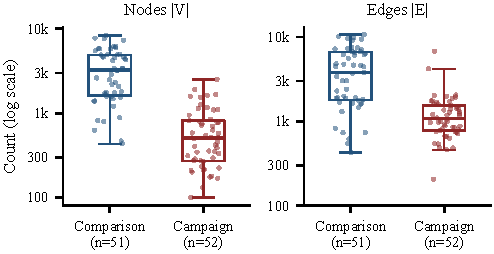
\includegraphics[width=\columnwidth]{figures/fig1_size_distributions.pdf}}
\caption{Event-graph size by class on a logarithmic axis. Left: node count; right: edge count. Boxes show interquartile ranges and medians; points are events (comparison $n=\RNComparison$, campaign $n=\RNCampaign$).}
\label{fig:sizes}
\end{figure}

\section{Methods}\label{sec:methods}
\subsection{Features and Conventions}\label{sec:features}
All features are computed per event graph $G=(V,E)$ with NetworkX~\cite{nx}. \emph{Counts} are $\log(1+|V|)$ and $\log(1+|E|)$. \emph{Degree concentration} is the Gini coefficient of the in-degree and of the out-degree sequence, where for a non-negative vector $x$ sorted in ascending order
\begin{equation}
G(x)=\frac{2\sum_{i=1}^{n} i\,x_{(i)}-(n+1)\sum_{i=1}^{n} x_{(i)}}{n\sum_{i=1}^{n} x_{(i)}}.
\label{eq:gini}
\end{equation}
\emph{Arrangement} comprises reciprocity, the fraction of nodes in the largest weakly connected component, and the median and maximum core number. Core numbers are computed on the simple undirected projection with self-loops removed ($\{u,v\}$ is an edge if $(u,v)$ or $(v,u)$ is, $u\neq v$); a node whose only edges are self-loops has core number 0. \emph{Content} comprises the exact-duplicate fraction of cleaned message texts, a Gini coefficient over message frequencies, and the standard deviation of message token counts. Density $|E|/(|V|(|V|-1))$ is a deterministic function of the counts. We therefore treat it as scale-encoding, not as topology, and use it only in a diagnostic model.

\subsection{Study 1: Feature Sets and Paired Inference}
Seven feature sets share identical event-level folds: M0, counts; M0q, counts with squared and interaction terms as a nonlinear count control; M1 = M0q + degree Gini; M2 = M1 + arrangement; M3 = M0q + content; M4 = M2 + content; and a diagnostic M4 + density. They form two nested chains, M0 $\subset$ M0q $\subset$ M1 $\subset$ M2 $\subset$ M4 $\subset$ M4 + density and M0q $\subset$ M3 $\subset$ M4; M3 is not nested in M1 or M2. Three primary contrasts were specified before the corrected run: C1 (M4 vs M0q, anything beyond counts), C2 (M2 vs M1, arrangement beyond degree concentration) and C3 (M3 vs M0q, content beyond counts). They were not preregistered, and an earlier version of this study had analysed the same archive. All other contrasts are exploratory.

Logistic regression (LR, with median imputation, standardization and balanced class weights) is the primary model~\cite{sklearn}; gradient-boosted trees (HGBT) are secondary. All hyperparameters are tuned by inner three-fold cross-validation inside each outer training fold; for LR, the regularization strength $C$ is chosen from $\{\RHOrigGrid\}$, and a wider grid is examined in Section~\ref{sec:rq1}. Balanced accuracy (BA) and log loss are distinct estimands with separately tuned fits: BA comes from fits tuned for BA, log loss from fits tuned for log loss, and the area under the ROC curve (AUC) is secondary. Differences are estimated on identical events with an event-level paired bootstrap of fixed out-of-fold predictions~\cite{efron} (\RNBoot{} resamples), and Holm correction is applied separately to the three BA and the three log-loss primary tests~\cite{holm}. These intervals do not include refitting or split variability~\cite{varoquaux}, which we report separately from \RNSplits{} fold splits, including the primary one; the splits are not independent replicates.

\subsection{Degree-Preserving Null}
To test arrangement beyond degree~\cite{maslov}, each graph is rewired by directed double-edge swaps $(a,b),(c,d)\to(a,d),(c,b)$ on non-loop edges, rejecting swaps that create self-loops or repeated edges; self-loops are held fixed. This preserves every node's in- and out-degree, $|V|$, $|E|$, density and the degree Gini coefficients exactly. It changed reciprocity in \RChRecipPct\% of events, the largest-component fraction in \RChWCCPct\% and the maximum core number in \RChCoreMaxPct\%, but the median core number in only \RChCoreMedPct\%, so it is a constrained degree-preserving comparison rather than a randomization of all graph structure. Directed double-edge swaps also do not reach every digraph with the given degrees, so this is not a uniform sample. We use \RSwaps{} swaps per edge and \RRealizations{} realizations per event, refit M2 with arrangement features from the rewired graphs, and compare it with M2 on the real graphs, both per realization and with the probabilities of the \RRealizations{} rewired fits averaged per event. Realizations are nested within events and are not independent samples.

\subsection{Exploratory Size Matching}
Campaign and comparison events are matched one-to-one on log node count with a caliper of \RCaliper{} standard deviations~\cite{austin,stuart}, giving \RPairs{} pairs (\RMatchedEvents{} events; signed SMD \RSMDBefore{} $\to$ \RSMDAfter, i.e., $|\mathrm{SMD}|$ \RAbsSMDBefore{} $\to$ \RAbsSMDAfter). Greedy matching depends on the order in which events are visited, and node-only matching does not balance edge counts. We therefore repeat it over \ROrders{} visiting orders, with and without edge count as a second matching variable, keeping pairs in the same fold.

\subsection{Study 2: Single-View Observation Design}
For $K\in\{250,500,1000\}$, every eligible event (at least $K$ edges) is reduced to $K$ uniformly sampled edges with ten sampling seeds per event, and every feature is recomputed from the sampled edges only. All conditions at a given $K$ use the same events, the full-cohort folds restricted to those events, and the same feature definitions: \emph{FF}, a model trained and evaluated on full graphs; \emph{FK}, the full-graph model applied to single $K$-edge views (frozen transfer); and \emph{KK}, a model trained and evaluated on single $K$-edge views from the same seed. The feature sets are the sampled endpoint count $\NK$ alone, six structural features (degree Gini, reciprocity, largest component and coreness), $\NK$ plus structure, and $\NK$ plus structure plus content. Density is excluded because at fixed $K$ it is determined by $\NK$:
\begin{equation}
D_K=\frac{K}{\NK(\NK-1)}.
\label{eq:density}
\end{equation}
The estimand is single-view performance, computed per sampling seed and averaged over seeds; the ensemble that averages probabilities over the ten views is reported separately. Study 2 is exploratory: its paired contrasts use an event-level bootstrap of the single-view estimand (\RSTwoNBoot{} resamples), with no correction for multiple comparisons. We report budget-specific cohorts ($K=250$: \REligTwoFifty{} events, \REligTwoFiftyCamp/\REligTwoFiftyComp; $K=500$: \REligFiveHundred, \REligFiveHundredCamp/\REligFiveHundredComp; $K=1000$: \REligThousand, \REligThousandCamp/\REligThousandComp) and a common cohort of the \REligThousand{} events eligible at every budget. $K=2000$ is infeasible for five-fold stratified evaluation because only \RTwoThousandCamp{} campaign events have at least 2,000 edges. To explain the sampled endpoint count, we use its expectation under uniform sampling of $K$ of the $m=|E|$ edges without replacement, where $d_v$ is the number of distinct edges incident to $v$:
\begin{equation}
\mathbb{E}[\NK]=\sum_{v\in V}\left[1-\binom{m-d_v}{K}\Big/\binom{m}{K}\right].
\label{eq:endpoints}
\end{equation}

\section{Results}\label{sec:results}
\subsection{Counts and Incremental Information (RQ1)}\label{sec:rq1}
Table~\ref{tab:levels} reports out-of-fold performance by feature level. Node and edge counts alone (M0, LR) reach BA \RCountsBA; node count alone reaches \RNodeOnlyBA. The full feature set M4 reaches BA \RAllBA, log loss \RAllLL{} and AUC \RAllAUC, against \RCountsQLL{} and \RCountsQAUC{} for the count model.

\begin{table}[htbp]
\caption{Out-of-Fold Performance by Feature Level ($N=\RNEvents$)}
\begin{center}
\footnotesize
\setlength{\tabcolsep}{3pt}
\begin{tabular}{|l|c|c|c|c|c|c|}
\hline
\textbf{Level} & \textbf{LR BA} & \textbf{\shortstack{LR\\log loss}} & \textbf{LR AUC} & \textbf{\shortstack{HGBT\\BA}} & \textbf{\shortstack{HGBT\\log loss}} & \textbf{\shortstack{HGBT\\AUC}} \\
\hline
\RTabLevels
\multicolumn{7}{p{0.92\columnwidth}}{\raggedright BA from BA-tuned fits; log loss and AUC from log-loss-tuned fits.}
\end{tabular}
\label{tab:levels}
\end{center}
\end{table}

The primary contrasts (Table~\ref{tab:contrasts}, Fig.~\ref{fig:contrasts}) separate the three measures. \textbf{For classification decisions, no contrast shows a detectable gain on the primary split.} C1, the difference in BA between all features and counts, is \RCOneBA{} \RCOneBACI, with \RCOneOnlyAll{} events classified correctly only by M4 and \RCOneOnlyCounts{} only by the count model. C2 and C3 are also indistinguishable from zero. These results are inconclusive, not evidence of equivalence: the intervals admit gains of up to about \RBAMaxHi. \textbf{For probability quality and ranking, the combined features help.} C1 improves log loss by \RCOneLLGain{} \RCOneLLCI{} (Holm $p=\RCOneLLHolm$) and AUC by \RCOneAUC{} \RCOneAUCCI. Neither arrangement beyond degree (C2) nor content alone (C3) accounts for this gain. In exploratory, uncorrected contrasts, M4 also changed log loss by \RETwoLL{} \RETwoLLCI{} against M3 and by \REThreeLL{} \REThreeLLCI{} against M2. Because LR is additive, this indicates complementary information in the combined feature set rather than a modelled interaction, and its source is not isolated. Log loss is a proper scoring rule that reflects both calibration and discrimination; we did not assess calibration separately.

\begin{table}[htbp]
\caption{Primary Paired Contrasts, LR: $\Delta$ [95\% CI] (Holm $p$)}
\begin{center}
\footnotesize
\setlength{\tabcolsep}{3pt}
\begin{tabular}{|l|c|c|c|}
\hline
\textbf{Contrast} & \textbf{$\Delta$BA} & \textbf{$\Delta$log loss} & \textbf{$\Delta$AUC} \\
\hline
\RTabContrasts
\end{tabular}
\label{tab:contrasts}
\end{center}
\end{table}

\begin{figure}[!t]
\centerline{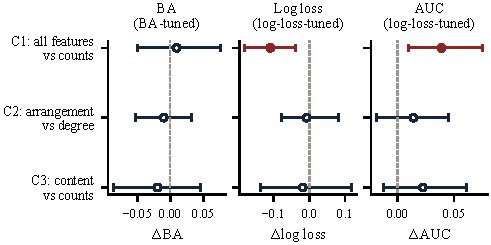
\includegraphics[width=\columnwidth]{figures/fig2_study1_contrasts.pdf}}
\caption{Primary paired contrasts (LR, $N=\RNEvents$). Points are differences A $-$ B on identical events; bars are 95\% event-level paired bootstrap intervals of fixed out-of-fold predictions. Filled red points exclude zero. Lower log loss is better.}
\label{fig:contrasts}
\end{figure}

The bootstrap intervals above resample events for one fixed set of out-of-fold predictions; fold-split variability is a different source of uncertainty, which we examine by refitting. Across \RNSplits{} fold splits, the C1 BA difference was positive in all \RSplitNWord{} (\RSplitBAMin{} to \RSplitBAMax, mean \RSplitBAMean), so the primary split shows the smallest gain; the C1 log-loss difference was negative in \RSplitLLNeg{} (\RSplitLLMin{} to \RSplitLLMax, median \RSplitLLMedian); and the C1 AUC difference ranged from \RSplitAUCMin{} to \RSplitAUCMax. The C2 and C3 BA differences changed sign across splits. Because the splits reuse the same events, these consistent signs are not independent replications and do not establish a reliable BA improvement. Hyperparameter selection was also sensitive to the order of events: re-running with permuted rows moved the C1 BA difference from \RRowOneStudy{} to \RRowOnePerm{} and the C3 BA difference from \RRowThreeStudy{} to \RRowThreePerm, while the C1 log-loss difference was unchanged (\RRowOneLL). The count models chose the largest $C$ of the grid in every log-loss fold. With $C$ widened to $\{\RHGridMin, \dots, \RHGridMax\}$, inner cross-validation chose weaker regularization for M0q, but its out-of-fold log loss rose from \RCountsQLL{} to \RHCountsLL, while that of M4 was \RHAllLL; C1 became \RHCOneLL{} \RHCOneLLCI{} for log loss (negative in \RHSplitLLNeg{} of \RSplitNWord{} splits) and \RHCOneBA{} \RHCOneBACI{} for BA. The count baseline's apparent under-tuning therefore did not explain its log-loss disadvantage. The wider grid does not resolve boundary effects for every model: the BA-tuned M0q and M2 fits and the log-loss-tuned M3 fit still chose its largest value in some folds. HGBT is secondary. Its own count model is weak (BA \RHGBTCountsBA), so gains measured within HGBT are inflated. Against the best count model (LR M0q), HGBT M4 changes BA by \RHGBTvsLRBA{} \RHGBTvsLRBACI{} and AUC (from log-loss-tuned fits, as elsewhere) by \RHGBTvsLRAUC{} \RHGBTvsLRAUCCI, and its log loss (\RHGBTAllLL) is worse than that of LR.

\subsection{Arrangement Beyond Degree}
Real graphs differ strongly from their rewired counterparts: the median observed-minus-null $z$-score for reciprocity is \RZRecipCamp{} in campaign and \RZRecipComp{} in comparison events, and about \RZWCCCamp{} for the largest-component fraction. These medians cover only events with a non-zero null spread; with \RRealizations{} realizations, the null standard deviation of reciprocity was zero, and its $z$-score undefined, in \RZUndefRecipPct\% of events. The arrangement features nevertheless showed no detectable improvement over the null. M2 on real graphs reached BA \RNullRealBA. Fitted separately on each rewired realization, M2 reached a mean BA of \RNullMeanBA{} (range \RNullMinBA--\RNullMaxBA); against the averaged probabilities of the \RRealizations{} rewired fits, the real-graph model differed by \RNullDBA{} \RNullDBACI{} in BA and \RNullDLL{} \RNullDLLCI{} in log loss (Table~\ref{tab:null}). These are different aggregations: against the per-realization mean, the real-graph model is \RNullMeanMinusReal{} lower, a difference without an interval. Neither comparison establishes equivalence, and neither shows that topology is uninformative. Mixing was limited. About \RUnmovedPct\% of non-loop edges per graph could not be moved (median), a plateau reached by five swaps per edge and concentrated in hub-dominated graphs, and because the median core number was almost never changed, the null mainly tests reciprocity, connectivity and the maximum core number.

\begin{table}[htbp]
\caption{Degree-Preserving Null (LR, $N=\RNEvents$)}
\begin{center}
\footnotesize
\setlength{\tabcolsep}{4pt}
\begin{tabular}{|>{\raggedright\arraybackslash}p{0.5\columnwidth}|c|}
\hline
\textbf{Quantity} & \textbf{Value} \\
\hline
\RTabNull
\multicolumn{2}{p{0.92\columnwidth}}{\raggedright\let\\\tabularnewline$^{\mathrm{a}}$BA of M2 fitted on each rewired realization separately. $^{\mathrm{b}}$Probabilities of the \RRealizations{} rewired fits averaged per event, compared with the real-graph fit by paired bootstrap; the two rows are different aggregations.}
\end{tabular}
\label{tab:null}
\end{center}
\end{table}

\subsection{Exploratory Size Matching}
Across \ROrders{} visiting orders, node-only matching retained \RPairsMin--\RPairsMax{} pairs but left edge counts imbalanced ($|\mathrm{SMD}|$ of log edge count \REdgeSMDMin--\REdgeSMDMax). Within matched cohorts, the count model fell to near chance (median BA \RMatchCountsBA), while the content model's point estimates stayed above 0.5 in every ordering (median \RMatchContentBA, range \RMatchContentMin--\RMatchContentMax; Table~\ref{tab:matching}). These are point estimates over visiting orders, without sampling intervals; with \RPairsMin--\RPairsMax{} pairs each is imprecise, so they are not evidence of above-chance performance, and matching also changes the evaluated population.

\begin{table}[htbp]
\caption{Exploratory Matching Sensitivity, LR BA: Median [Range] over Visiting Orders}
\begin{center}
\footnotesize
\setlength{\tabcolsep}{3pt}
\begin{tabular}{|>{\raggedright\arraybackslash}p{0.2\columnwidth}|c|c|c|c|}
\hline
\textbf{Matching} & \textbf{Pairs} & \textbf{M0 counts} & \textbf{M3 content} & \textbf{M4 all} \\
\hline
\RTabMatching
\end{tabular}
\label{tab:matching}
\end{center}
\end{table}

\subsection{Restricted Observation (RQ2)}
Table~\ref{tab:singleview} and Fig.~\ref{fig:singleview} report single-view BA. On the same events, a model trained and evaluated on single $K$-edge views (KK) with all features was not detectably less accurate than the full-graph model with all features (FF): the single-view minus full-graph BA difference was \RViewMinusFullTwoFifty{} \RViewMinusFullTwoFiftyCI{} at $K=250$, \RViewMinusFullFiveHundred{} \RViewMinusFullFiveHundredCI{} at $K=500$ and \RViewMinusFullThousand{} \RViewMinusFullThousandCI{} at $K=1000$ (Table~\ref{tab:stwocontrasts}), with log-loss differences of \RViewMinusFullLLTwoFifty{} \RViewMinusFullLLTwoFiftyCI, \RViewMinusFullLLFiveHundred{} \RViewMinusFullLLFiveHundredCI{} and \RViewMinusFullLLThousand{} \RViewMinusFullLLThousandCI. At these budgets, sampling did not detectably reduce the label information available on the evaluated cohorts. The positive BA difference at $K=1000$ is an exploratory, uncorrected result on a small, imbalanced cohort (\REligThousand{} events, \REligThousandCamp/\REligThousandComp) whose log-loss difference includes zero; it does not indicate that sampling generally improves classification. $\NK$ alone and structure alone did not differ detectably ($\NK$ minus structure: \RNKMinusStructTwoFifty{} \RNKMinusStructTwoFiftyCI, \RNKMinusStructFiveHundred{} \RNKMinusStructFiveHundredCI, \RNKMinusStructThousand{} \RNKMinusStructThousandCI); adding $\NK$ to structure changed BA by \RNKAddedTwoFifty{} \RNKAddedTwoFiftyCI, \RNKAddedFiveHundred{} \RNKAddedFiveHundredCI{} and \RNKAddedThousand{} \RNKAddedThousandCI. Content added at most a few points of BA, with intervals that include zero at every budget.

The training regime mattered more than any feature choice we tested. With the same six structural features, events and folds, training on single views instead of applying the full-graph model raised single-view BA at $K=250$ (budget-specific cohort, $n=\RNViewEvents$) by \RRetrainTwoFifty{} \RRetrainTwoFiftyCI, and by \RRetrainFiveHundred{} and \RRetrainThousand{} at $K=500$ and 1000. With all features, the corresponding changes were \RRetrainAllTwoFifty{} \RRetrainAllTwoFiftyCI, \RRetrainAllFiveHundred{} \RRetrainAllFiveHundredCI{} and \RRetrainAllThousand{} \RRetrainAllThousandCI, the last interval including zero. Applying the full-graph model to views lost \RTransferLossTwoFifty{} BA at $K=250$ relative to full graphs, a loss whose interval includes zero at larger budgets. Averaging the ten views changed BA by at most \REnsembleMax{} in the budget-specific cohorts, so ensembling contributes little. On the common cohort of the \RCommonN{} events eligible at every budget, the retraining, transfer, feature and ensembling contrasts have the same directions at $K=250$ and 500 (for example, a $K=250$ retraining effect of \RCommonRetrainTwoFifty), although on this cohort the content interval at $K=500$ excludes zero; an exploratory diagnostic of density in frozen models changed sign between cohorts and is not interpreted.

\begin{table}[htbp]
\caption{Single-View Balanced Accuracy (Budget-Specific Cohorts)}
\begin{center}
\footnotesize
\setlength{\tabcolsep}{4pt}
\begin{tabular}{|l|c|c|c|}
\hline
\textbf{Condition (feature set)} & \textbf{$K=250$} & \textbf{$K=500$} & \textbf{$K=1000$} \\
\hline
\RTabSingleView
\multicolumn{4}{p{0.92\columnwidth}}{\raggedright Mean over 10 sampling seeds. FF rows use the full graphs of the same events (no sampling); the last row averages probabilities over the 10 views.}
\end{tabular}
\label{tab:singleview}
\end{center}
\end{table}

\begin{figure}[!t]
\centerline{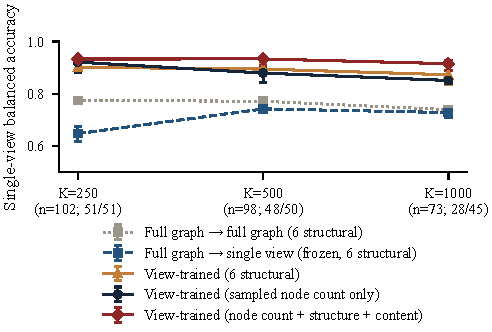
\includegraphics[width=\columnwidth]{figures/fig3_study2_single_view.pdf}}
\caption{Single-view balanced accuracy by edge budget on the common cohort ($n=\RCommonN$; \RCommonCamp/\RCommonComp), the events eligible at every budget, so that every line compares the same events; full-graph (FF) values do not depend on $K$. Points are means over 10 sampling seeds and bars span the minimum and maximum over seeds; they are not confidence intervals. Table~\ref{tab:singleview} reports the budget-specific cohorts.}
\label{fig:singleview}
\end{figure}

\begin{table}[htbp]
\caption{Study 2 Paired Contrasts (Exploratory), Single-View $\Delta$BA [95\% CI]}
\begin{center}
\footnotesize
\setlength{\tabcolsep}{2.5pt}
\begin{tabular}{|>{\raggedright\arraybackslash}p{0.22\columnwidth}|c|c|c|}
\hline
\textbf{Contrast} & \textbf{$K=250$} & \textbf{$K=500$} & \textbf{$K=1000$} \\
\hline
\RTabSTwoContrasts
\multicolumn{4}{p{0.92\columnwidth}}{\raggedright Budget-specific cohorts. Event-level paired bootstrap (\RSTwoNBoot{} resamples); no multiplicity correction.}
\end{tabular}
\label{tab:stwocontrasts}
\end{center}
\end{table}

\subsection{What the Sampled Endpoint Count Reflects}\label{sec:endpoints}
The expectation in~\eqref{eq:endpoints} matches the observed mean $\NK$ within \RMechRelErr\% at $K=250$ and agrees with a Monte Carlo check on three events. It carries strong label information: at $K=250$ its AUC is \RMechAUC, compared with \RMechAUCNodes{} for full-graph log node count. The expected number of distinct endpoints in a fixed-budget edge sample is strongly associated with full-graph node count and mean degree. Together, these variables explain \RRTwoSizeDegree\% of its variation at $K=250$ in the analysed archive (node count alone: \RRTwoNodes\%). Adding in/out-degree Gini provides no measurable additional explanatory power (\RRTwoWithGini\% with it). Because~\eqref{eq:endpoints} depends on the full incidence-degree distribution, these aggregates describe, but do not completely determine, the quantity (Fig.~\ref{fig:mechanism}). Within sampled views, the six structural features also predict $\log\NK$ closely: a linear regression, cross-validated with events grouped, reaches $R^2$ of \RProxyRTwoTwoFifty, \RProxyRTwoFiveHundred{} and \RProxyRTwoThousand{} at $K=250$, 500 and 1000. The endpoint count and the structural features therefore carry largely overlapping, size-like information, and this analysis does not establish that $\NK$, rather than structure, is responsible for the predictive signal.

\begin{figure}[!t]
\centerline{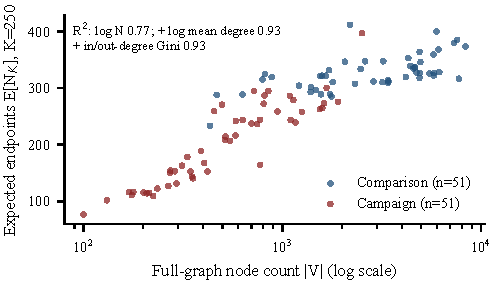
\includegraphics[width=\columnwidth]{figures/fig4_endpoint_mechanism.pdf}}
\caption{Expected distinct endpoints in a 250-edge sample, from~\eqref{eq:endpoints}, against full-graph node count for the \REligTwoFifty{} eligible events. Inset: variance of $\log\mathbb{E}[\NK]$ explained by log node count, by log node count and log mean degree, and additionally by in/out-degree Gini.}
\label{fig:mechanism}
\end{figure}

\section{Discussion}\label{sec:discussion}
On this archive, the released labels are predictable to a large degree from how large an event graph is. Counts reach most of the BA reached by the evaluated models, and richer features did not produce a detectable improvement in classification decisions; the BA point estimate was small and positive in every fold split examined, which is not evidence of a reliable gain. They did improve probability quality and ranking, which matters when scores are used directly or thresholds are chosen after deployment, but the source of this gain is not isolated. Anyone using LEN-Small as a benchmark should read reported accuracy against a count-only baseline and report probabilistic metrics separately.

The null-model result is narrow by design. The real graphs are far from degree-preserving random graphs, so their arrangement is not random; the tested arrangement features simply showed no detectable improvement over the degree sequences for the model we used. Other arrangement statistics, other null models or larger cohorts could change this.

Under restricted observation, a single view was not detectably less informative than the full graph with the same features. Much of that information is size-like: the number of distinct endpoints a view touches, a quantity strongly associated with the full graph's node count and mean degree, is itself closely encoded by the structural features. A model needs to be trained on observations like those it will see: frozen transfer from full graphs loses accuracy at small budgets, while averaging many views adds almost nothing.

These results do not establish that any model detects coordinated behavior, accounts or intent, that size is the only relevant property, or any causal effect. They concern one released archive, which differs from the official release.

\section{Limitations}\label{sec:limitations}
\emph{Sample size and uncertainty.} With \RNEvents{} events, null BA results are inconclusive rather than evidence of equivalence. Paired intervals resample fixed out-of-fold predictions and exclude refitting and split variability; re-drawn splits show C1 differences that vary in magnitude, and the primary split shows the smallest C1 BA gain of the \RSplitNWord. Hyperparameter selection in small inner folds was sensitive to row order and, for log loss, to the width of the regularization grid.

\emph{Provenance.} The archive has \RNEvents{} events rather than the official \ROfficialN, for an unknown reason. Labels come from file names. Account identifiers and campaign subtypes are not available, so dependence between events through shared accounts and heterogeneity across subtypes cannot be assessed. \RHashtagPairsCap{} campaign hashtags each appear as two events on nearby dates, and \RHashtagPairsSplit{} pair falls in different folds, so not every event is independent of the others. LEN-Small itself is selected by node count, so associations between size and label in this archive need not hold in the full LEN dataset. Timestamp semantics are unverified, so temporal features are excluded.

\emph{Null model and matching.} Rewiring mixes incompletely in hub-dominated graphs, leaves the median core number almost unchanged and uses only \RRealizations{} realizations, too few to estimate the null spread reliably. Matching keeps \RPairsMin--\RPairsMax{} pairs, changes the evaluated population, does not balance all size measures and is reported without sampling intervals.

\emph{Scope of models and observations.} Only LR and HGBT on hand-crafted features were evaluated. Graph neural networks and the methods of~\cite{len,decode} were not re-run, and published LEN-Small accuracies use a different protocol and metric. Uniform edge sampling is one observation mechanism among many~\cite{leskovec}, and the Study 2 contrasts are exploratory and uncorrected for multiplicity.

\section{Methodological Corrections}\label{sec:corrections}
Validation of an earlier version of this analysis identified two errors, both corrected before the results reported here were produced.

\emph{Coreness and self-loops.} Every graph in the archive contains self-loops, which the core-number routine does not accept. The earlier implementation set both coreness features to zero instead of failing, so its arrangement features carried no coreness information. Core numbers are now computed on the undirected projection without self-loops (Section~\ref{sec:features}). The error affected every model that uses arrangement features.

\emph{Fold assignment for frozen models.} In the frozen-transfer evaluation, sampled events were assigned to fold models with a split specific to each edge budget instead of the full-cohort split, so some events were scored by a model whose training data included their own full graph. Such leakage inflates frozen-transfer accuracy. Each sampled event is now scored only by the full-cohort fold model that held it out. The error affected only the frozen-transfer condition.

Both corrections are covered by regression tests, and every result in this paper comes from the corrected pipeline. The superseded outputs are retained in the project repository, with their values, for reference.

\section{Conclusion}\label{sec:conclusion}
First, LEN-Small's labels, as distributed in the analysed archive, are highly predictable from graph size, although we do not show that size is the only relevant property. Second, additional degree, arrangement and content features improved probability quality and ranking without a reliable improvement in balanced accuracy, and the tested arrangement features showed no detectable improvement over a degree-preserving null. Third, under fixed-budget observation, the sampled endpoint count and the structural features encode substantially overlapping, size-like information; single views were not detectably less informative than full graphs on the evaluated cohorts, and training on matching observations mattered far more than ensembling. Evaluations on this benchmark should report count-only baselines, separate decision and probability metrics, and match training to the observation regime. Natural next steps are to obtain the official release and account-level data to test provenance and dependence, and to evaluate learned graph models under the same paired protocol.

\section*{Code and Data Availability}
Source code, configuration files, tests, derived event-level outputs and reproduction instructions are available at \url{https://github.com/SynshAmi/temporal-coordination-in-social-media}. The code is released under the MIT licence, which does not extend to this paper, its figures or any data. One command runs the pipeline from the raw archive to every number, table and figure in this paper, with seeds fixed for folds, matching, edge sampling, rewiring and bootstrap. An independent verification script recomputes all reported comparisons from the saved predictions (\RChecksPassed{} of \RChecksTotal{} checks pass), including checks that permuting held-out labels leaves the tuned hyperparameters unchanged. A complete rerun from the raw archive reproduced every reported value on the original machine; reproduction on other hardware has not been tested. LEN is released by its authors under a CC-BY licence~\cite{len}. We do not redistribute the raw LEN-Small archive, which must be obtained from the LEN project~\cite{repo}. The repository records the SHA-256 digest of the archive analysed here; its derived files (event names, counts, file digests, features and predictions) are shared with attribution for reproducibility and are not endorsed by the LEN authors.

\bibliographystyle{IEEEtran}
\bibliography{references}

\end{document}
